\chapter{Results}
\label{chap:results}

\begin{figure}
    \centering
    \begin{subfigure}[t]{0.45\textwidth}
        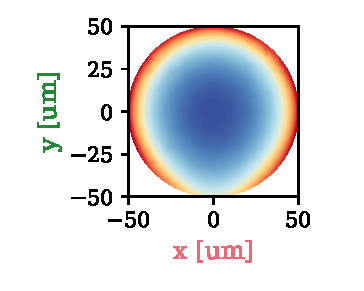
\includegraphics{figures/magnetic_field_distribution_in_trap_horizontal.pdf}
        \caption{Magnetic flux density norm in the xy-plane for $z = 0$.}
        \vfill
    \end{subfigure}
    \hfill
    \begin{subfigure}[t]{0.45\textwidth}
        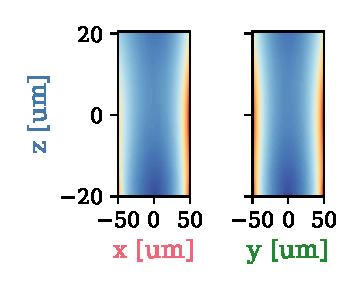
\includegraphics{figures/magnetic_field_distribution_in_trap_vertical.pdf}
        \caption{Magnetic flux density norm in the $xz$- and $yz$-plane for $y = 0$ and $x=0$ respectively.}
    \end{subfigure}
    \caption{A simulation of the magnetic flux density norm (\unit{\tesla}) inside of the trap for $\chi = -2$. The magnitude of the color scale is arbitrary. Blue corresponds to low magnetic field density and red to high magnetic field density. The assymetry of the magnetic field in the $y$-direction is due to the assymetry of the trap.}
    \label{fig:magnetic_field_distribution_in_trap}
\end{figure}

\begin{figure}
    \centering
    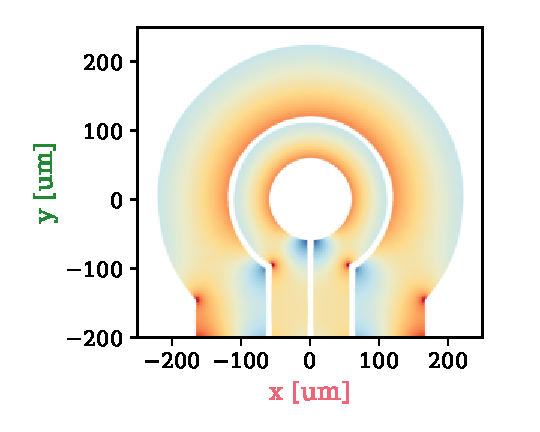
\includegraphics{figures/current_through_tracks.pdf}
    \caption{A simulation of the current density norm (\unit{\ampere\per\square\meter}) inside of the tracks for $\chi = -2$. The magnitude of the color scale is arbitrary. Blue corresponds to low current density and red to high current density. The extremely low and high current densities in the sharp corners are simulation artefacts. The current concentrates itself on the inside of the tracks.}
    \label{fig:current_through_tracks}
\end{figure}
